\chapter{Particle Physics}
\label{chap:particlephysics}

Particle physics is the study of the elementary particles and fundamental forces
of nature. By ``elementary particles'' we mean the smallest, most
basic building blocks of all structures in the universe. By
``fundamental forces'' we mean the basic kinds of interactions between
particles, from which all other known interactions in the universe
arise.

This chapter will provide a simple introduction to the concepts
and terminology of particle physics, with the dual goals of motivating the
research in this dissertation, and of making that research understandable to
readers inexperienced in particle physics. Pursuant to those
goals, this introduction will focus on the concepts most relevant to
the research, and will use plain, non-technical language as much as
possible. These self-imposed constraints risk hiding some of the
considerable beauty and richness of particle physics, so I encourage the
interested reader to seek deeper explanations elsewhere.

\section{The Standard Model}
\label{sec:standardmodel}

\subsection{Description}
\label{ssec:SM:description}

The Standard Model (SM) is the scientific theory that describes
(almost) all the particles and forces we know of and their properties.
It is a relativistic quantum field theory, describing both the
behavior of particles at speeds up to and including the speed of
light, as well as their quantum mechanical nature.
The Standard Model was developed beginning in the early 1970s,
through the joint efforts of theoretical and experimental physicists.
Although it is not a perfect description of all known physical
phenomena, it has correctly predicted numerous discoveries,
cementing its place as one of the most
successful physical theories of all time \cite{griffiths,smcoffee}.

The Standard Model describes two families of matter particles -- that is
to say, particles that may give rise to tangible structures at the macro scale.
These two families are called quarks and leptons. In addition, it
describes several force-carrying particles, as well as the Higgs
boson. A sort of ``periodic table'' of these particles is given in
Figure \ref{fig:standardmodel}. A diagram showing which particles
interact with which other particles is given in Figure \ref{fig:couplings}.

\begin{figure}[h]
  \centering
  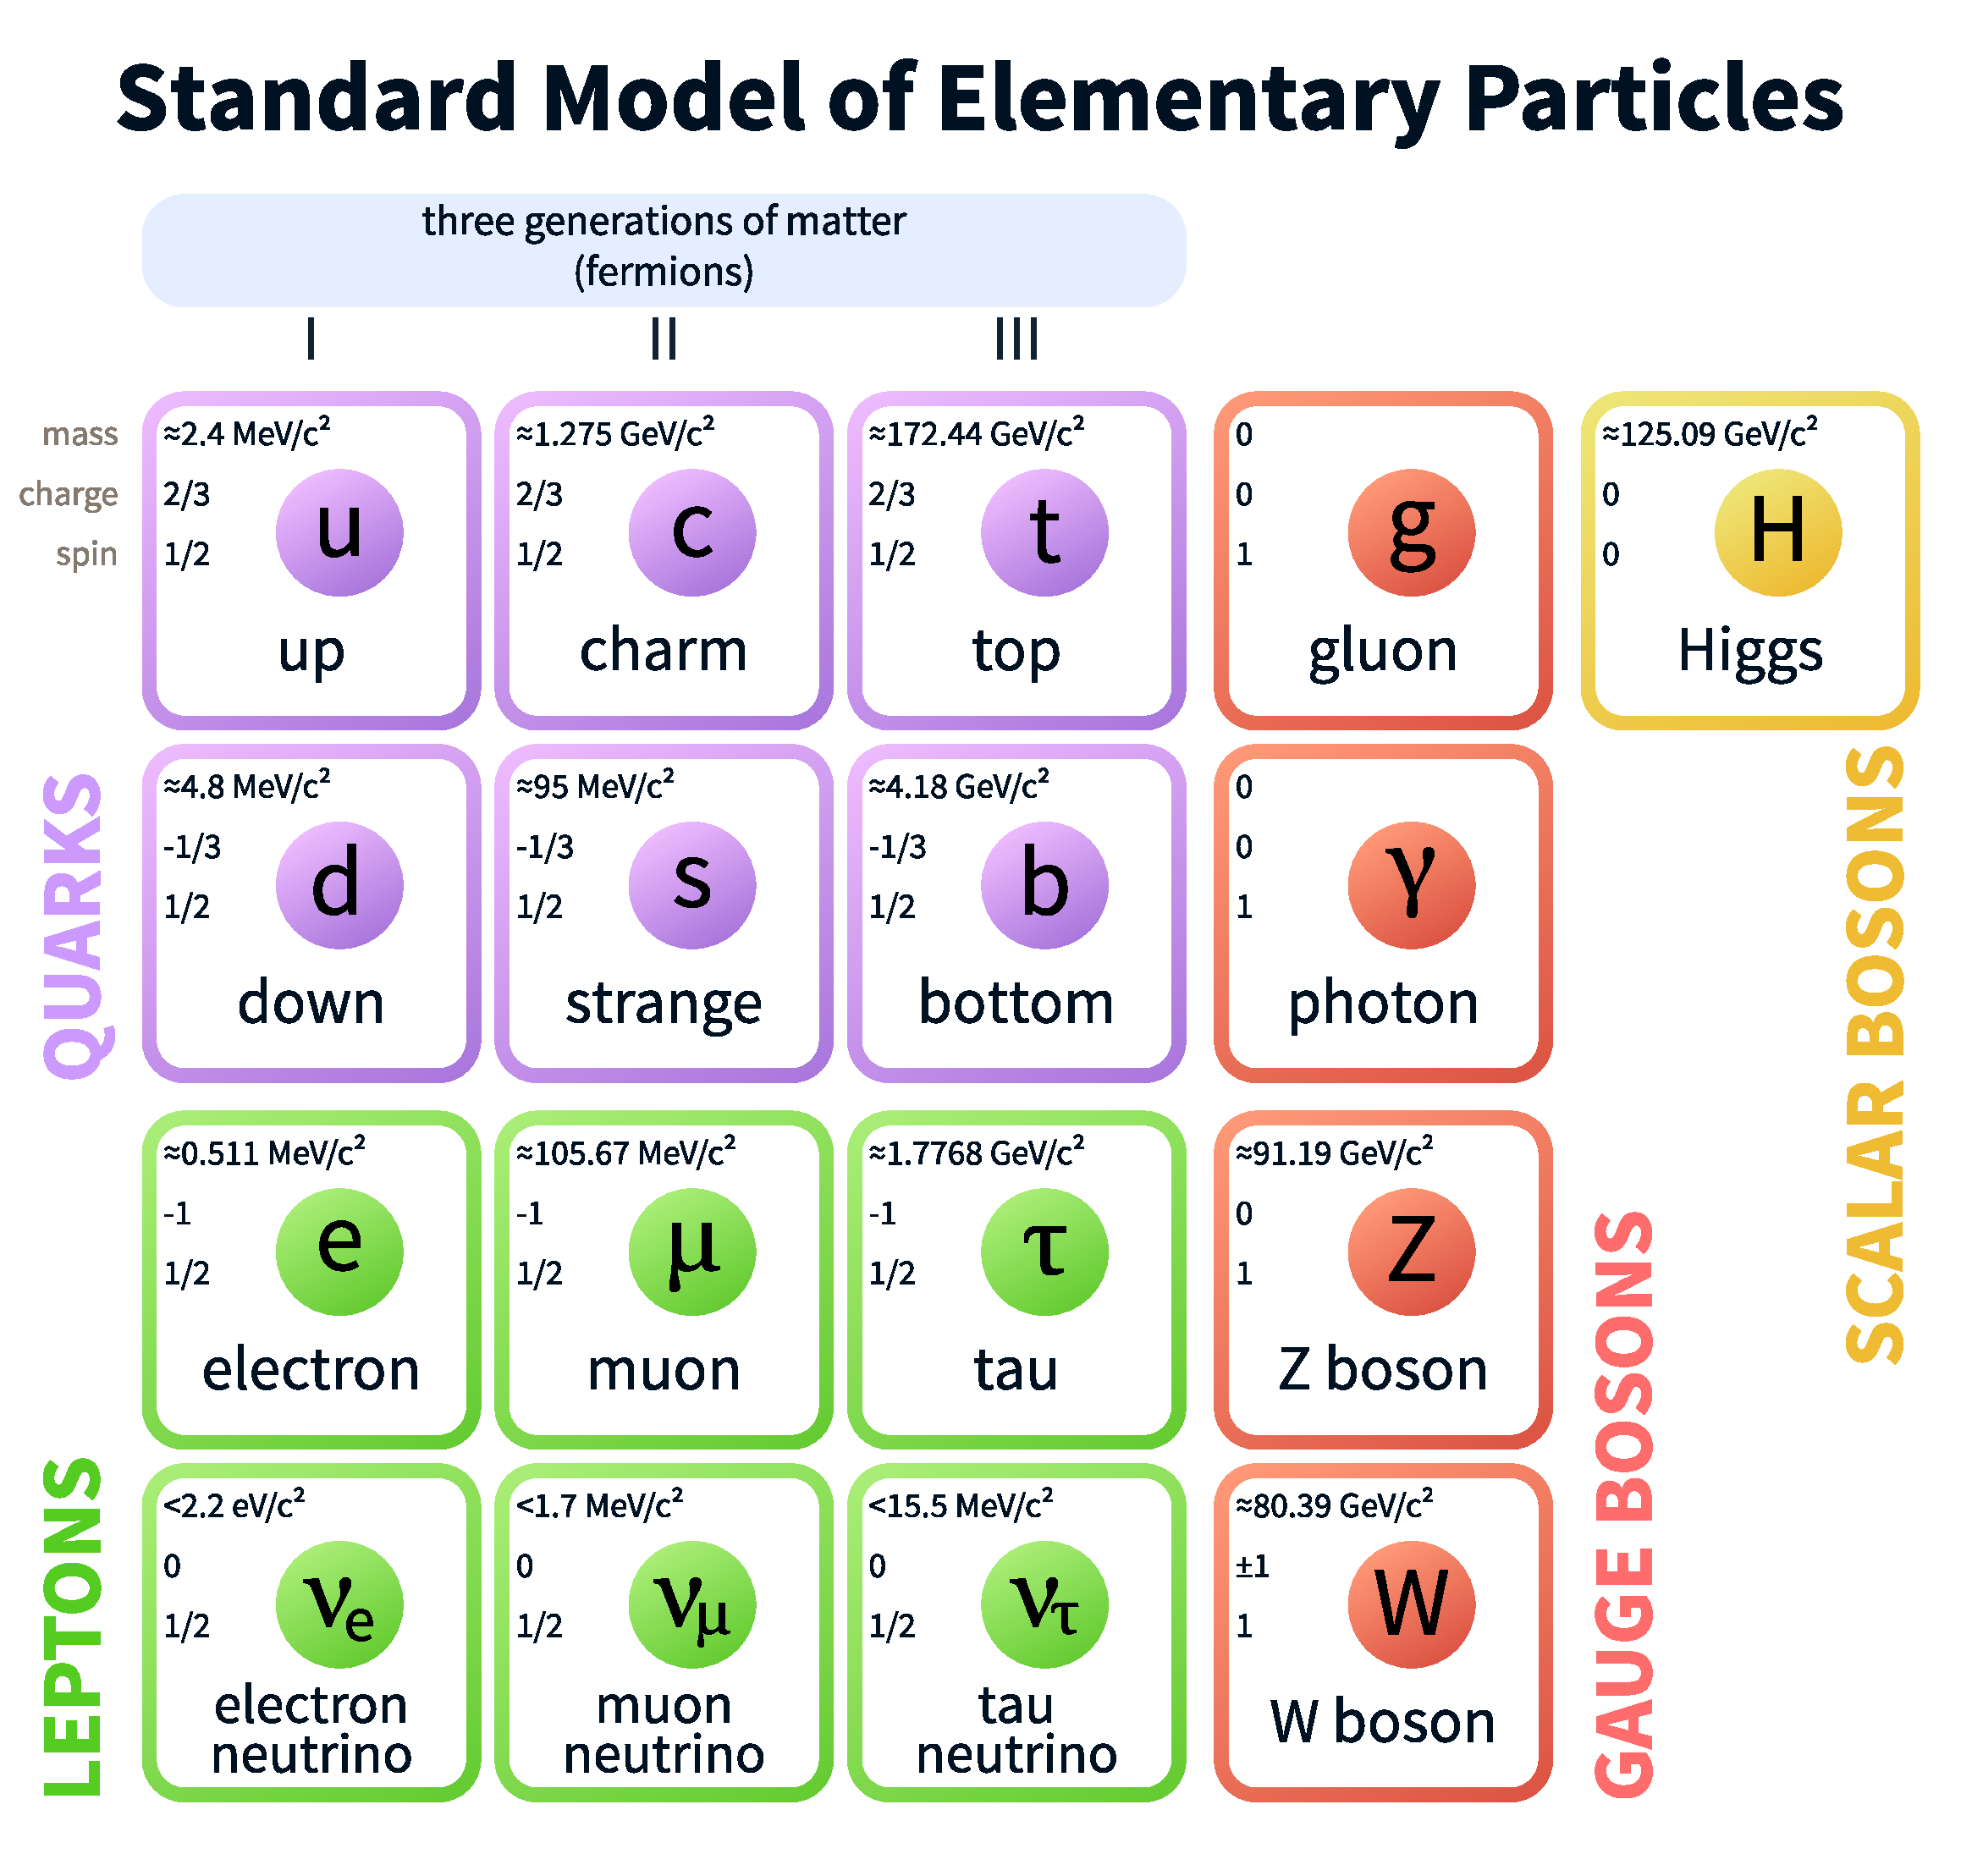
\includegraphics[width=0.75\textwidth]{figures/standard-model-light.pdf}
  \caption%[A diagram of all the particles of the Standard Model,
          %grouped into families of related particles.]
  {A diagram of all the particles of the Standard Model, grouped into
  families of related particles. Mass measurements are constantly
  being improved, and the listed mass values may not reflect the latest and
  best measurements.}
  \label{fig:standardmodel}
\end{figure}

\subsubsection*{Quarks}
There are six quarks in the SM. In order from lightest to heaviest,
these quarks are named \emph{up, down, strange, charm, bottom,} and
\emph{top}. They are often referred to using only the first letter of
their names. Up and down quarks are essential to our lives, as
they make up the nuclei of atoms: ignoring short-lived quantum
fluctuations, the proton is composed of two up
quarks and a down quark bound together ($uud$), and the neutron is composed of one up
quark and two down quarks bound together ($udd$). The four heavier
quarks tend to decay into lighter quarks within a fraction of a
second, so they are generally not found in everyday matter. The up,
charm, and top quarks all have a positive charge with $\frac{2}{3}$ the
magnitude of the electron's charge, and the down, strange, and bottom
quarks have a negative charge that is $\frac{1}{3}$ that of the electron.

The top quark has several unique properties that make it important
in particle physics. Not only is
it the heaviest quark, but it is also the heaviest elementary particle
we know of, with a measured mass of approximately 173 giga-electron
volts (GeV). This figure is comparable to the mass
of an entire tungsten atom, which contains a multitude of quarks and
electrons. For comparison, the mass of the up quark is only about
2.2 mega-electron volts (MeV) \cite{pdg}.
In addition, when the top quark decays, it has a 96\% chance of
decaying into a bottom quark and a W boson \cite{pdg}. Few other
particles have such predictable decay products. The reasons why these
properties are so important will be articulated in later chapters. % Reference a more specific section once written?

\subsubsection*{Leptons}
There are three defining members of the lepton family. In order of
increasing mass, they are: the electron
($e^-$), the muon ($\mu^-$), and the tau ($\tau^-$). As their symbols
denote, these leptons each have a negative electric charge. They are
often referred to collectively as the charged leptons.
The electron is well known as the part of an atom responsible for the
majority of its chemical interactions with other atoms. Muons and taus
tend to decay within a fraction of a second, so they also tend not to
be found in everyday matter. However, muons are often produced in
Earth's upper atmostphere due to bombardment by cosmic rays (particles
streaming in from outer space) \cite{griffiths}.

For each charged lepton, there is a corresponding particle called a
neutrino. They are the electron neutrino ($\nu_e$), the muon
neutrino ($\nu_{\mu}$), and the tau neutrino ($\nu_{\tau}$). As their
name suggests, neutrinos are electrically neutral - they have no
charge. In addition, neutrinos have extremely small masses. In fact,
the SM considers them to be massless particles, but experimental
results show they have non-zero masses of less than one electron volt
(eV) \cite{pdg}. Neutrinos also have an extremely small probability of
interacting with matter. In practice, this makes neutrinos
difficult or impossible to detect. The experimental implications of
this fact will be described in chapter \ref{chap:hardware}. % Reference a more specific section once written?

\begin{figure}[h]
  \centering
  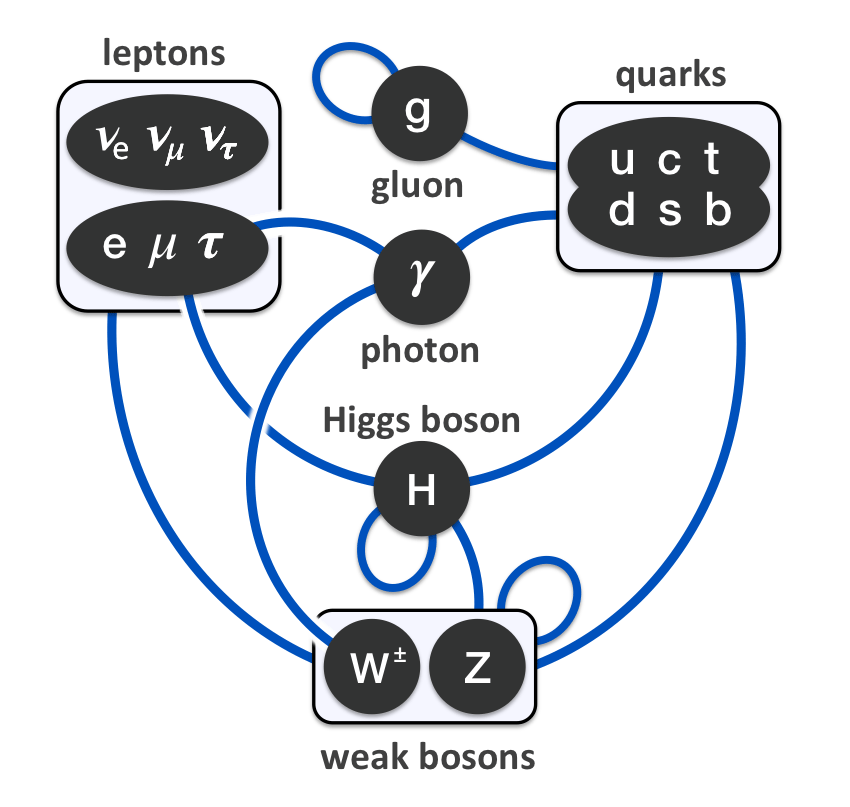
\includegraphics[width=0.75\textwidth]{figures/couplings.png}
  \caption{A diagram of the interactions, or couplings,
    between the particles of the Standard Model. Particles or groups
    of particles connected by blue lines are able to interact with
    each other.}
  \label{fig:couplings}
\end{figure}

\subsubsection*{Force Carriers}
The Standard Model describes four force-carrying particles. These
particles are the physical manifestations, or \emph{quanta}, of the forces
they convey. In general, matter particles interact with other matter
particles through the force-carriers. However, not all particles are
able to interact with all forces.

% Do I need to explain Feynman diagrams?
% If so, this might be a good place to do it.

The photon ($\gamma$), commonly known as the particle of light,
is in fact the quantum of the electromagnetic
force. Thus every time two particles interact electrically or
magnetically, they do so by exchanging photons. Only particles that
have a non-zero electric charge can interact electromagnetically. Thus
we say the photon \emph{couples to} charged particles. All quarks, as
well as the charged leptons, carry electric charge. The photon travels
at the speed of light, and has no mass or electric charge.

The gluon ($g$) is the carrier of the strong nuclear force. The strong
force is responsible for binding together quarks to form protons,
neutrons, and other composite particles (known collectively as
\emph{hadrons}). This same interaction also causes protons and neutrons to
bind together into atomic nuclei. Gluons couple to any particle
that has so-called \emph{color charge}, namely quarks and
other gluons. Although gluons are in principle massless, the energy of
their collective interactions actually makes up more than 98\% of the
mass of protons and neutrons \cite{protonmass}.

The W and Z bosons ($W^+$, $W^-$, $Z$) carry the weak nuclear force. This
force is best known for mediating radioactive $\beta$-decay through
the W bosons. In addition, the W boson mediates all Standard Model
processes where a quark or lepton changes flavor \cite{griffiths}.
Particle physicists know the Z boson best for its
role in the Drell-Yan process, where pairs of quarks convert into
pairs of charged leptons. The W and Z bosons couple to all matter
particles. In addition, they are capable of coupling to each other,
though such interactions are rare. The W bosons have a mass of around
80 GeV, and the Z boson has a mass around 91 GeV \cite{pdg}.

\subsubsection*{Higgs Boson}
The Higgs boson is neither a force-carrying particle nor a matter particle, but
something else entirely. It is the manifestation, or quantum, of the
Higgs field, a field that permeates the entire universe, and endows
mass upon most elementary particles. The top quark is so massive
because it couples very strongly to the Higgs field. Similarly, the
photon is massless because it does not couple to the Higgs field at all.
The Higgs boson was discovered in 2012, and measured to have a mass
of about 125 GeV \cite{jointhiggs}. Thus the Higgs must also couple to itself.

\subsubsection*{Spin}
All particles (both elementary and composite) have
a property known as spin. Spin is an intrinsic property, just like
mass or electric charge. But unlike those properties, spin is quantum
mechanical in nature. So a particle's spin is sometimes called its
spin quantum number. All particles can be divided into two categories
based on their spin quantum numbers: particles whose spin is an
integer (0, 1, 2, 3,$\ldots$) are called \emph{bosons}, and particles whose
spin is a half-integer ($\frac{1}{2}, \frac{3}{2}, \frac{5}{2},\ldots$)
are called \emph{fermions}. Figure \ref{fig:standardmodel}
labels which particles are fermions and which are bosons, but even
absent those labels, you could see that quarks and leptons are all
fermions because they have spins of $\frac{1}{2}$, and the force
carriers and the Higgs particle are all bosons.

\subsubsection*{Antimatter}
For every matter particle, there also exists a corresponding
antiparticle. These are collectively referred to as
antimatter. Antiparticles have mostly the exact same properties as
their normal-matter partners, the key exception being that their electrical charge (if
they have one) is opposite in sign. Thus the anti-electron (also
called a positron) has a positive electrical charge instead of
negative. The antimatter versions of the charged leptons are indicated
with a plus in their symbol ($e^+, \mu^+, \tau^+$), and all other
antiparticles have a bar on top of their symbol ($\bar{u},
\bar{b}, \bar{\nu_{\mu}}$, etc.). Since the properties of
antiparticles are mostly identical to those of normal-matter
particles, particle physicists seldom distinguish between matter and
antimatter in our speech or writing.

When a particle meets its own antiparticle, they usually annihilate,
and produce high-energy photons, or sometimes Z bosons. Because of this
instant annihilation, antimatter is not generally found
in large quantities in our universe. However, very small quantities can be
produced by energetic collisions in nature, radioactive decays, and in manmade
particle colliders.

\subsection{Successes}
\label{ssec:SM:successes}

The predictions of the Standard Model have been borne out in a
staggering number of experiments over the last several decades.
Some of the greatest successes of the SM
include the correct predictions of the Higgs boson, the W and Z
bosons, and the top and bottom quarks. On a less exciting but equally
telling note, thousands of deliberate searches for phenomena that
violate the Standard Model have been conducted by a wide variety of
experimental groups; the overwhelming majority have failed to find
any such violations. This unprecedented success has led the
Standard Model to be labeled as one of the most successful
physics theories ever formulated \cite{griffiths,smcoffee}.

\subsection{Shortcomings}
\label{ssec:SM:shortcomings}

Despite the Standard Model's vast successes, it is not a complete
theory of all particles and interactions in the universe. Physicists
have observed a number of phenomena that are not described within the
framework of the Standard Model. Additionally, the Standard Model does
not contain all the information needed to build a stable universe from
scratch. Some of these shortcomings are presented here, as they provide
strong motivations for further research in particle physics and
related fields.

\subsubsection*{Gravity and the Hierarchy Problem}
When describing the fundamental forces of nature in Section
\ref{ssec:SM:description}, one force was conspicuous by its absence:
gravity. Although gravity is the most apparent force of nature in our
everyday lives, and was the first to be described mathematically,
the Standard Model is still unable to incorporate the workings of
gravity. Einstein's general theory of relativity does a marvelous job
describing gravity on the scale of large objects, such as stars or
galaxies. However, physicists have so far been unable to formulate a
theory of gravity consistent with quantum mechanics, a necessary step
to incorporate gravity into the Standard Model.

One key stumbling block in the quest to quantize gravity (though by no
means the only one) is called the Hierarchy Problem. In plain language, the
problem is that gravity is weaker than the other fundamental forces by
a staggering 20 to 30 orders of magnitude, depending on the distance
scale considered. Any attempt to unite gravity and the other forces
of nature must find a way to bridge this gulf. % Do I need a citation here?

\subsubsection*{Arbitrary Parameters}
Another perceived deficit of the Standard Model is the fact that many
of the fundamental constants of nature are not given in the theory. For
example, the Standard Model predicts the existence of the elementary
particles described in Sec. \ref{ssec:SM:description}, but it does
not predict what their masses will be;
the masses must be measured experimentally. Similarly, the Standard
Model offers no clue to the strength of the various forces of nature,
only their existence. In total, the Standard Model has 19 independent
parameters that cannot be derived from other information in the theory
\cite{smparams}. Some physicists object to this large number as being clunky
and inelegant, feeling that a fundamental description of the universe
should have fewer unexplained parameters \cite{griffiths}.

\subsubsection*{Dark Matter}
Humans have been observing the motions of stars
for millenia. Starting in the late 19\textsuperscript{th}
century, scientists attempted to calculate the mass of the Milky Way
galaxy based on the stars and gas they could see through their
telescopes. They soon discovered that the galactic mass estimated from
visible matter was significantly less than the galactic mass
estimated from Newtonian gravity and the velocities of those objects. In the early
20\textsuperscript{th} century, astronomers began to notice the same
discrepancy for distant galaxies and galaxy clusters as well \cite{dmhistory}.
They hypothesized that galaxies contained some kind of
matter that was not visible through telescopes (hence \emph{dark}),
but that nevertheless exerted a gravitational pull.
In fact, we now estimate that only about $\frac{1}{6}$ of the
mass of the universe consists of visible matter such as stars
and planets, and the remainder consists of this mysterious dark matter
\cite{planck2013}.

Since everything is made of particles, the particle physics community
is naturally curious to learn what particles make up dark matter.
The observation that dark matter neither absorbs nor emits light
indicates that it does not interact electromagnetically, and thus
cannot be charged. Observations of distant stars, and calculations of
nucleus formation after the Big Bang, have ruled out the possibility
that dark matter is made of baryons (three-quark hadrons,
such as the proton and neutron). Finally, simulations have shown
that neutrinos could not give rise to the large-scale structures
we see in the universe \cite{dmhistory}.
This exhausts all possibilities from among standard-model particles.
Therefore, the existence of dark matter seems to require
physics Beyond the Standard Model (BSM).

\subsubsection*{Dark Energy}
In a universe filled with ordinary matter and dark matter, it is
natural to believe that the inexorable pull of gravity would
slow the expansion of that universe, until the universe eventually began to
contract again. However, observations of the cosmic microwave background
(CMB), distant supernovae, galaxy clusters, and more have shown that
the expansion of the universe is \emph{accelerating}, not slowing
\cite{darkenergy}. The mysterious energy that drives this outward expansion
is given the name ``dark energy''. Thus far, the Standard Model offers no
explanation for how this kind of energy could exist.

\subsubsection*{Neutrino Masses and Oscillations}
The Standard Model predicts that neutrinos should be entirely
massless. And for many years, observations of processes that produced
neutrinos, such as $\beta$-decay, seemed to confirm this
belief. However, beginning in 1968, observations of neutrinos produced in
the sun showed that the rate of electron neutrinos reaching the earth
was only a third of what was expected \cite{homestake1968,homestake1992}.
Further measurements of neutrinos from the sun, nuclear reactors, and
particle accelerators eventually led to the conclusion that neutrinos
change back and forth between their three flavors as they
travel through space \cite{nuphenom}. This mutability makes it impossible
for neutrinos to be massless, because massless particles must travel
at the speed of light, and therefore cannot experience the passage of
time. But since neutrinos morph between different states, clearly they
must have some experience of time passing. These
oscillations require an extension of the Standard Model to
explain how neutrinos acquire mass, and how they are able to
change identities.

\section{Supersymmetry}
\label{sec:susy}

Physicists have proposed a number of theories to explain the various
shortcomings of the Standard Model. One particular class of theories,
known as supersymmetry (or SUSY for short), is extremely popular for
the elegant ways it can fill some of these gaps. Although there
are numerous variations of supersymmetric theories, they all have one
defining feature in common. For every standard-model particle, SUSY
postulates the existence of another particle with mostly the same
properties, but with a spin that differs by $\frac{1}{2}$. Thus every standard-model
fermion would have a corresponding ``superpartner'' that is a boson,
and every standard-model boson would have a superpartner that is a
fermion \cite{susyprimer}.

% Consider inserting, somewhere near here, a picture of the
% SM+SUSY. Something that shows the relationship between particles and sparticles.

\subsection{Sparticles}
\label{ssec:susy:sparticles}

Supersymmetry uses a unique, sometimes quirky nomenclature to refer to
the new particles it postulates. The partners of Standard Model
fermions are named by prefixing the existing name with an `s'. Thus
the two families become \emph{squarks} and \emph{sleptons}, and the
individual members of those families are named, e.g., \emph{sup,
  sbottom, selectron, sneutrino}, etc. Meanwhile the partners of
Standard Model bosons gain the suffix \emph{-ino}, which replaces the
suffix \emph{-on} if present. Thus we arrive at the names
\emph{gluino, photino, Zino, Wino}, and \emph{Higgsino}. The symbols
for these particles are generally formed by adding a tilde on top of
the original particle's symbol, so that a scharm squark is notated
$\tilde{c}$, a gluino is notated $\tilde{g}$, etc. To avoid conflict
with the tilde, anti-sparticles are notated using a prime (as in
$\tilde{c}^\prime$) instead of a bar.

These superpartners are capable of mixing with each other to form
different sparticles, which may not correspond exactly to Standard
Model particles. Of particular note are the neutralinos
($\lsp_1, \lsp_2, \lsp_3, \lsp_4$), made by mixing the photino, zino,
and Higgsino; and the charginos ($\chargino_1, \chargino_2$), made by
mixing charged Winos and charged Higgsinos.

It is worth noting that if SUSY were a perfect symmetry, all
sparticles would have the same masses as their corresponding
particles. However, to date, no sparticles have been
observed, implying that most sparticles (if they exist) must be too
heavy to produce using our current particle colliders. Since the
equality of masses is destroyed, we say SUSY is a \emph{broken
symmetry} \cite{susyprimer}.

\subsection{Rationale}
\label{ssec:susy:rationale}

One of the features that makes SUSY very attractive is its ability to
solve the hierarchy problem. The exact nature of this solution
invokes complicated physics, but it revolves around
the notion that the introduction of several new massive sparticles
creates substantial corrections to the square of the mass of the
Higgs boson ($m_H^2$) \cite{susyprimer}.
% However, the essence is
% that the massive Standard Model particles should make the Higgs mass
% squared ($m_H^2$) blow up to an enormous value; by introducing a
% new boson for every SM fermion, and vice-versa, SUSY cancels out
% the effects of the SM particles, and allows $m_H^2$ to take on a
% more reasonable value \cite{susyprimer}.

In addition, SUSY provides particles that may be good candidates to
explain dark matter. At the moment, the most popular explanation for
the composition of dark matter is weakly-interacting massive particles
(WIMPs). These are particles that primarily interact through the weak
force, and that also have mass, allowing them to exert a gravitational
pull. The neutralinos fit this bill nicely. In addition, the dark
matter particle must be stable. The lightest supersymmetric particle
(LSP) would be stable due to conservation laws associated
with supersymmetry. In fact, many SUSY models predict that the lightest
neutralino, $\lsp_1$, actually \emph{is} the LSP. Thus the lightest
neutralino makes a tantalizing dark matter candidate
\cite{susydarkmatter,susyprimer}. We will assume moving forward
that $\lsp_1$ is the LSP, and will use the terms LSP and neutralino
interchangeably.

If the theoretical considerations were not enough to make SUSY an
attractive target for study, there is a strong experimental case as
well. \emph{Naturalness} is the idea that it makes sense for the
parameters of a model to be not-too-dissimilar in size (the hierarchy
problem is an example of un-naturalness). If SUSY is
to be ``natural'', as many theorists hope it is, then the lightest
sparticles are likely to have masses in the terra-electron volt (TeV)
range \cite{susydarkmatter,susyprimer}. This is exactly the energy
scale probed by current and near-future collider experiments.
Therefore, there is reason to believe that searches at the Large Hadron
Collider or a close successor must uncover evidence for the existence
of supersymmetry.
